\documentclass[a4paper,11pt]{article}
\usepackage{xcolor}
\usepackage{tikz}
%\usepackage{tkz-euclide}
\usetikzlibrary{shapes.geometric, arrows.meta}
 \tikzstyle{startstop} = [rectangle, rounded corners, minimum width=3cm, minimum height=1cm,text centered, draw=black]
\tikzstyle{process} = [rectangle, minimum width=3cm, minimum height=1cm, text centered, text width=3cm, draw=black]
\tikzstyle{decision} = [diamond, minimum width=4cm,  text centered, draw=black]
\tikzstyle{arrow} = [thick,->,>=Latex]
\begin{document}
\begin{figure}[h!]
\begin{center}
 \scalebox{0.85}{
 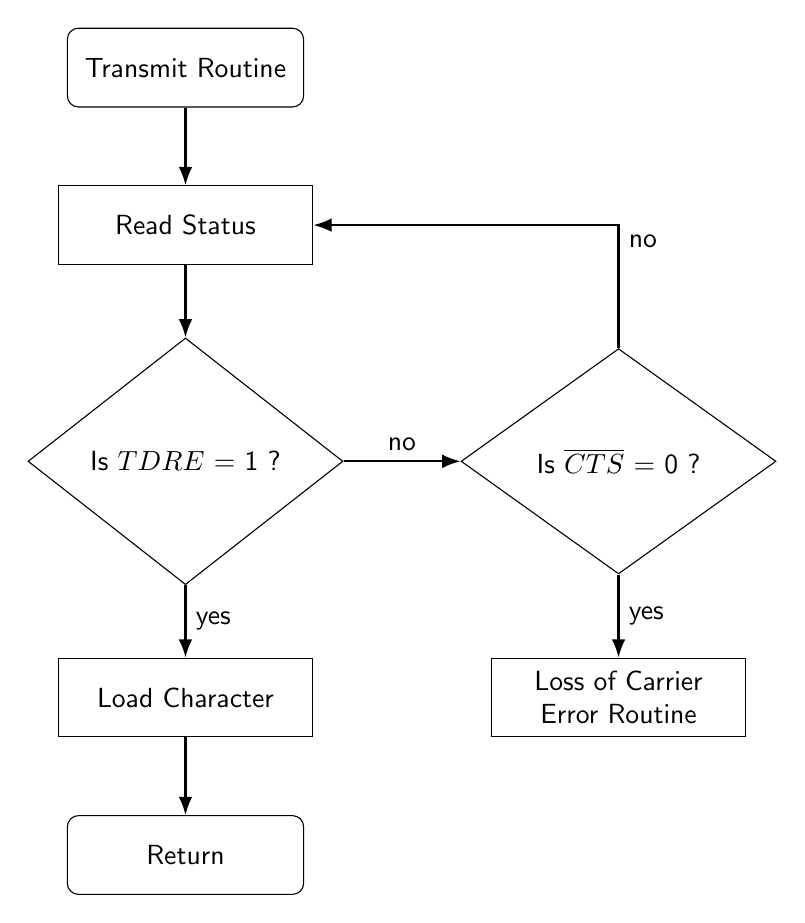
\begin{tikzpicture}[font=\sffamily,node distance=2cm]
	\node (start) [startstop] {Transmit Routine};
	\node (status) [process, below of=start] {Read Status};
	\node (tdre) [decision, below of=status, yshift=-1cm] {Is $TDRE$ = 1 ?};
	\node (load) [process, below of=tdre, yshift=-1cm] {Load Character};
	\node (rts) [startstop, below of=load] {Return};
	\node (cts) [decision, right of=tdre, xshift=3.5cm] {Is $\overline{CTS}$ = 0 ?};
	\node (error) [process, below of=cts, yshift=-1cm] {Loss of Carrier Error Routine};

	\draw [arrow] (start) -- (status);
	\draw [arrow] (status) -- (tdre);
	\draw [arrow] (tdre) -- node[anchor=west] {yes} (load);
	\draw [arrow] (load) -- (rts);
	\draw [arrow] (tdre) -- node[anchor=south] {no} (cts);
	\draw [arrow] (cts) |- node[anchor=north west] {no} (status);
	\draw [arrow] (cts) -- node[anchor=west] {yes} (error);
 \end{tikzpicture}
 }
 \caption{Transmit subroutine.}
 \label{fig:flowctl}
\end{center}
\end{figure}
\end{document}



